\chapter*{Zeitplan}


\begin{sidewaysfigure}[!ht]
    \centering
    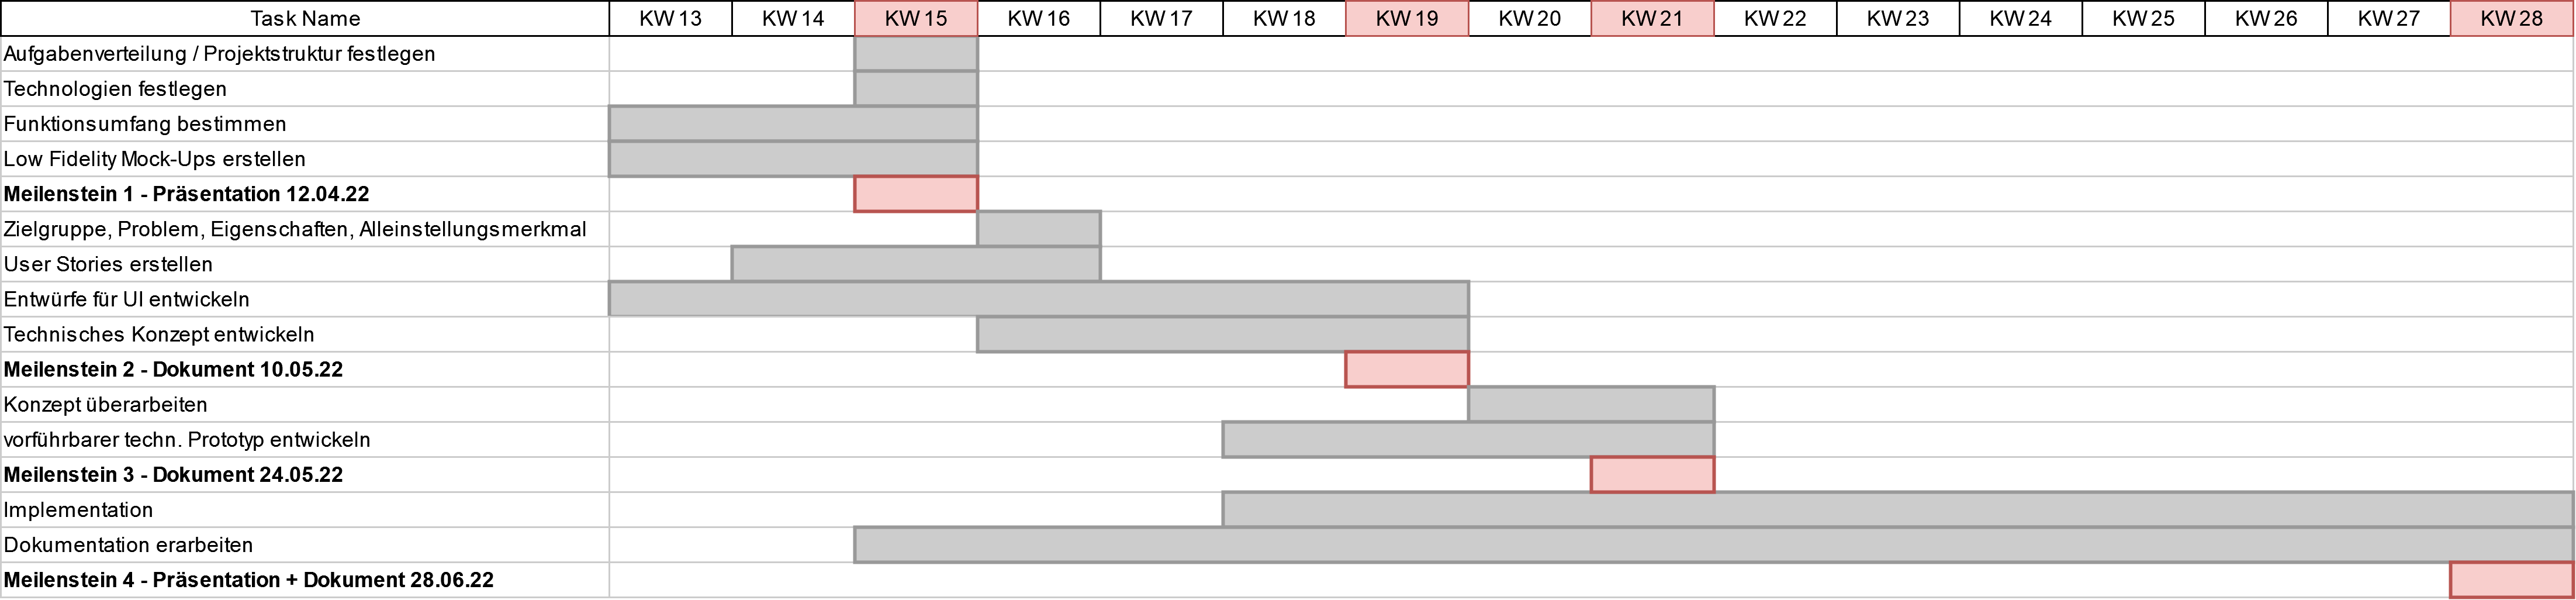
\includegraphics[width=1\textwidth]{Zeitplan_DeskPlanner.png}
    \caption{Zeitplan}
    \label{fig:Zeitplan}
\end{sidewaysfigure}

Der Zeitplan hangelt sich an den vorgegebenen Meilensteinen 1-4 entlang.
\\
\\
\textbf{Meilenstein 1 (12.04.22)}\\
Präsentation:
\begin{itemize}
    \item Aufgabenverteilung
    \item Projektmanagement
    \item Technologien
    \item Funktionsumfang
    \item UI-Entwürfe, z.B. Low Fidelity Mock-Ups
\end{itemize}

\vspace{0.03\textwidth}
\textbf{Meilenstein 2 (10.05.22)} \\
Dokumentation:
\begin{enumerate}
    \item Zielgruppe, Problem, Eigenschaften, Alleinstellungsmerkmal
    \item User Stories
    \item User Interface Entwürfe
    \item Technisches Konzept
    \begin{itemize}
        \item Verwendete Frameworks
        \item Softwarearchitektur
        \begin{itemize}
            \item UML-Verteilungsdiagramm des Gesamtsystems
            \item UML-Komponentendiagramm (jeweils für Client und Server)
        \end{itemize}
        \item Datenbank
        \begin{itemize}
            \item Entity Relationship Model
        \end{itemize}
    \end{itemize}
    \item UI-Entwürfe, z.B. Low Fidelity Mock-Ups
\end{enumerate}

\vspace{0.1\textwidth}

\textbf{Meilenstein 3 (24.05.22)} \\
Dokumentation: 
\begin{itemize}
    \item Überarbeiten und ergänzen Sie das Konzept von Meilenstein 2
\end{itemize}
Technischer Prototyp: 
\begin{itemize}
    \item Entwickeln Sie einen vorführbaren technischen Prototypen inkl. Login.
    \item Bereit halten für Code Reviews: Jedes Teammitglied muss einen Code-Teil \\präsentieren können
\end{itemize}


\textbf{Meilenstein 4 (28.06.22)}\\
Dokumentation erweitern:\\
\begin{itemize}
    \item Installations- und Administrationshandbuch
    \item Aufteilung des Teams: wer hat was gemacht (mit Namen der Teilnehmer)?
    \item Reflektion Projektmanagement: vergleichen Sie Ihre erste Planung mit der \\ tatsächlichen Durchführung; vergleichen Sie die Aufwandsschätzungen mit den \\realen Aufwänden;
    \item Reflektion Lernfortschritt: was haben Sie gelernt?
    \item Lizenzen: verwendete Lizenzen (Fremdcode: Frameworks, Libraries), unter \\ welche Lizenz stellen Sie Ihren Codes zur evtl. Weiterverwendung
    \item Ausblick: was könnte an Ihrem Projekt ergänzt werden?
\end{itemize}

\textbf{Abschlusspräsentation}